%% Creator: Inkscape 1.2.2 (b0a8486541, 2022-12-01), www.inkscape.org
%% PDF/EPS/PS + LaTeX output extension by Johan Engelen, 2010
%% Accompanies image file 'Figures/Objective_2/pvalue-matrix_2.pdf' (pdf, eps, ps)
%%
%% To include the image in your LaTeX document, write
%%   \input{<filename>.pdf_tex}
%%  instead of
%%   \includegraphics{<filename>.pdf}
%% To scale the image, write
%%   \def\svgwidth{<desired width>}
%%   \input{<filename>.pdf_tex}
%%  instead of
%%   \includegraphics[width=<desired width>]{<filename>.pdf}
%%
%% Images with a different path to the parent latex file can
%% be accessed with the `import' package (which may need to be
%% installed) using
%%   \usepackage{import}
%% in the preamble, and then including the image with
%%   \import{<path to file>}{<filename>.pdf_tex}
%% Alternatively, one can specify
%%   \graphicspath{{<path to file>/}}
%% 
%% For more information, please see info/svg-inkscape on CTAN:
%%   http://tug.ctan.org/tex-archive/info/svg-inkscape
%%
\begingroup%
  \makeatletter%
  \providecommand\color[2][]{%
    \errmessage{(Inkscape) Color is used for the text in Inkscape, but the package 'color.sty' is not loaded}%
    \renewcommand\color[2][]{}%
  }%
  \providecommand\transparent[1]{%
    \errmessage{(Inkscape) Transparency is used (non-zero) for the text in Inkscape, but the package 'transparent.sty' is not loaded}%
    \renewcommand\transparent[1]{}%
  }%
  \providecommand\rotatebox[2]{#2}%
  \newcommand*\fsize{\dimexpr\f@size pt\relax}%
  \newcommand*\lineheight[1]{\fontsize{\fsize}{#1\fsize}\selectfont}%
  \ifx\svgwidth\undefined%
    \setlength{\unitlength}{578.92927515bp}%
    \ifx\svgscale\undefined%
      \relax%
    \else%
      \setlength{\unitlength}{\unitlength * \real{\svgscale}}%
    \fi%
  \else%
    \setlength{\unitlength}{\svgwidth}%
  \fi%
  \global\let\svgwidth\undefined%
  \global\let\svgscale\undefined%
  \makeatother%
  \begin{picture}(1,0.83623286)%
    \lineheight{1}%
    \setlength\tabcolsep{0pt}%
    \put(0,0){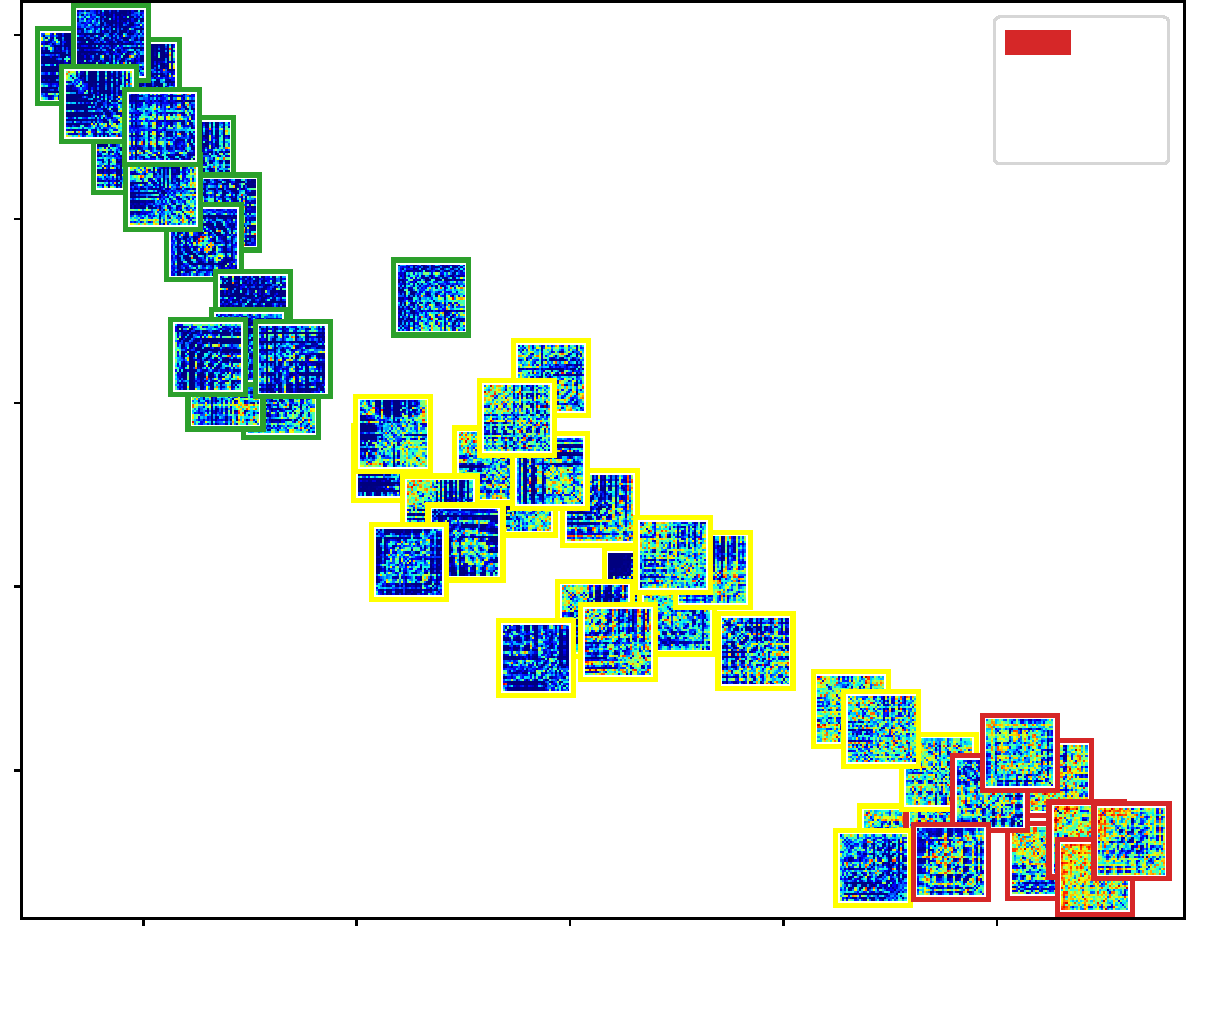
\includegraphics[width=\unitlength,page=1]{Figures/Objective_2/pvalue-matrix_2.pdf}}%
    \put(0.90737781,0.7925477){\color[rgb]{0,0,0}\makebox(0,0)[lt]{\lineheight{1.25}\smash{\begin{tabular}[t]{l}G.III\end{tabular}}}}%
    \put(0,0){\includegraphics[width=\unitlength,page=2]{Figures/Objective_2/pvalue-matrix_2.pdf}}%
    \put(0.90737781,0.75451951){\color[rgb]{0,0,0}\makebox(0,0)[lt]{\lineheight{1.25}\smash{\begin{tabular}[t]{l}G.II\end{tabular}}}}%
    \put(0,0){\includegraphics[width=\unitlength,page=3]{Figures/Objective_2/pvalue-matrix_2.pdf}}%
    \put(0.90737781,0.71649134){\color[rgb]{0,0,0}\makebox(0,0)[lt]{\lineheight{1.25}\smash{\begin{tabular}[t]{l}G.I\end{tabular}}}}%
    \put(0,0){\includegraphics[width=\unitlength,page=4]{Figures/Objective_2/pvalue-matrix_2.pdf}}%
    \put(-0.00115551,0.00028681){\color[rgb]{0,0,0}\makebox(0,0)[lt]{\lineheight{1.25}\smash{\begin{tabular}[t]{l}0.00\end{tabular}}}}%
    \put(0,0){\includegraphics[width=\unitlength,page=5]{Figures/Objective_2/pvalue-matrix_2.pdf}}%
    \put(0.0470369,0.00028681){\color[rgb]{0,0,0}\makebox(0,0)[lt]{\lineheight{1.25}\smash{\begin{tabular}[t]{l}0.05\end{tabular}}}}%
    \put(0,0){\includegraphics[width=\unitlength,page=6]{Figures/Objective_2/pvalue-matrix_2.pdf}}%
    \put(0.09522932,0.00028681){\color[rgb]{0,0,0}\makebox(0,0)[lt]{\lineheight{1.25}\smash{\begin{tabular}[t]{l}0.10\end{tabular}}}}%
    \put(0,0){\includegraphics[width=\unitlength,page=7]{Figures/Objective_2/pvalue-matrix_2.pdf}}%
    \put(0.19161414,0.00028681){\color[rgb]{0,0,0}\makebox(0,0)[lt]{\lineheight{1.25}\smash{\begin{tabular}[t]{l}0.20\end{tabular}}}}%
    \put(0,0){\includegraphics[width=\unitlength,page=8]{Figures/Objective_2/pvalue-matrix_2.pdf}}%
    \put(0.28799897,0.00028681){\color[rgb]{0,0,0}\makebox(0,0)[lt]{\lineheight{1.25}\smash{\begin{tabular}[t]{l}0.30\end{tabular}}}}%
    \put(0,0){\includegraphics[width=\unitlength,page=9]{Figures/Objective_2/pvalue-matrix_2.pdf}}%
    \put(0.38438379,0.00028681){\color[rgb]{0,0,0}\makebox(0,0)[lt]{\lineheight{1.25}\smash{\begin{tabular}[t]{l}0.40\end{tabular}}}}%
    \put(0,0){\includegraphics[width=\unitlength,page=10]{Figures/Objective_2/pvalue-matrix_2.pdf}}%
    \put(0.48076862,0.00028681){\color[rgb]{0,0,0}\makebox(0,0)[lt]{\lineheight{1.25}\smash{\begin{tabular}[t]{l}0.50\end{tabular}}}}%
    \put(0,0){\includegraphics[width=\unitlength,page=11]{Figures/Objective_2/pvalue-matrix_2.pdf}}%
    \put(0.57715344,0.00028681){\color[rgb]{0,0,0}\makebox(0,0)[lt]{\lineheight{1.25}\smash{\begin{tabular}[t]{l}0.60\end{tabular}}}}%
    \put(0,0){\includegraphics[width=\unitlength,page=12]{Figures/Objective_2/pvalue-matrix_2.pdf}}%
    \put(0.67353827,0.00028681){\color[rgb]{0,0,0}\makebox(0,0)[lt]{\lineheight{1.25}\smash{\begin{tabular}[t]{l}0.70\end{tabular}}}}%
    \put(0,0){\includegraphics[width=\unitlength,page=13]{Figures/Objective_2/pvalue-matrix_2.pdf}}%
    \put(0.7699231,0.00028681){\color[rgb]{0,0,0}\makebox(0,0)[lt]{\lineheight{1.25}\smash{\begin{tabular}[t]{l}0.80\end{tabular}}}}%
    \put(0,0){\includegraphics[width=\unitlength,page=14]{Figures/Objective_2/pvalue-matrix_2.pdf}}%
    \put(0.86630792,0.00028681){\color[rgb]{0,0,0}\makebox(0,0)[lt]{\lineheight{1.25}\smash{\begin{tabular}[t]{l}0.90\end{tabular}}}}%
    \put(0,0){\includegraphics[width=\unitlength,page=15]{Figures/Objective_2/pvalue-matrix_2.pdf}}%
    \put(0.96269275,0.00028681){\color[rgb]{0,0,0}\makebox(0,0)[lt]{\lineheight{1.25}\smash{\begin{tabular}[t]{l}1.00\end{tabular}}}}%
    \put(0,0){\includegraphics[width=\unitlength,page=16]{Figures/Objective_2/pvalue-matrix_2.pdf}}%
  \end{picture}%
\endgroup%
